\documentclass[11pt,a4paper]{article}
\usepackage[margin=2.2cm]{geometry}
\usepackage[T1]{fontenc}
\usepackage[utf8]{inputenc}
\usepackage{lmodern,microtype}
\usepackage{amsmath,amssymb,mathtools,bm}
\usepackage{booktabs,longtable,tabularx,array}
\usepackage{tikz}
\usetikzlibrary{arrows.meta,positioning,shapes.geometric}
\usepackage{xcolor,hyperref,cleveref,enumitem,fancyhdr,titlesec}
\usepackage{algorithm,algpseudocode}

\hypersetup{colorlinks=true,linkcolor=blue!55!black,citecolor=blue!55!black,urlcolor=blue!55!black}
\pagestyle{fancy}\fancyhf{}\lhead{MMALS G2}\rhead{Geometric Perspective v0.2-internal}\cfoot{\thepage}
\setlength{\parindent}{0pt}\setlength{\parskip}{0.65em}\setlength{\headheight}{14pt}
\newcommand{\MMALS}{\textsc{MMALS}}
\newcommand{\Chronicle}{\textsc{Chronicle}}
\newcommand{\CAL}{\textsc{MMALS-CAL}}
\newcommand{\TPUT}{\textsc{TPUT}}
\newcommand{\RCtwoO}{\textsc{RC2O}}
\newcommand{\M}{\mathcal{M}}
\newcommand{\status}[1]{\par\noindent\fbox{\begin{minipage}{0.94\linewidth}\textbf{Evidence status:} #1\end{minipage}}\par}
\newcommand{\R}{\mathbb{R}}
\title{\bfseries MMALS G2: A Geometric Perspective on Continual Functional Memory\\[0.4em]\large From Chronicle and inferred-context routing to admissible adaptation flows}
\author{Guillaume Harbonnier\\MMALS Research Programme}
\date{17 July 2026 -- Internal research snapshot v0.2}
\begin{document}
\maketitle
\begin{center}
\fbox{\begin{minipage}{0.94\linewidth}
\textbf{Internal archive notice.} This document freezes Guillaume Harbonnier's current MMALS G2 reflection state for private GitHub archiving and context recovery. It is not an external publication, a completed specification, or a safety claim. The final chapter is intentionally personal and records publication recommendations, unresolved hypotheses, and the release-gate plan.
\end{minipage}}
\end{center}
\begin{abstract}
This paper proposes the G2 geometric perspective for Mycelium-Inspired Mutualistic Adaptive Learning Systems (\MMALS). It starts from the evidence discipline established in Geometry-\MMALS~G1, the route-first control model of \RCtwoO/\TPUT, the dual reconstructive--compiled memory of \Chronicle, and the safety role of \CAL. It interprets continual learning not merely as sequential optimization, but as controlled transport of functions, routes, memories, and audit distributions across coupled geometric spaces. The selected paper by Perez-Dattari et al. on Stable Flow Matching Dynamical Systems supplies a decisive engineering pattern: expressive learned dynamics should be restricted to admissible velocity sets and stabilized either softly or by construction. G2 adapts that pattern cautiously. It does not assert that learning trajectories are physical trajectories, nor that a valid Lyapunov function already exists for arbitrary continual adaptation. Instead, it defines falsifiable geometric objects, candidate invariants, admissible transition cones, route--function alignment measures, and an experiment programme for testing whether geometric control adds value beyond non-geometric baselines under matched budgets.
\end{abstract}
\textbf{Keywords:} continual learning, inferred context, functional memory, routing geometry, information geometry, Lyapunov stability, flow matching, conformal prediction, engineering assurance.
\tableofcontents
\newpage

\section{Research boundary and central thesis}
G2 is not the claim that neural learning literally follows a physical manifold, nor that every adaptation can be assigned a conserved energy. It is the narrower proposition that the operational state of a continual adaptive system can be represented by geometric objects whose distances, tangent directions, transport maps, and admissible regions predict or improve behaviour under matched budgets.

\begin{quote}
A continual learner becomes engineerable when context inference, route selection, functional memory, adaptation, and safety calibration are treated as coupled but non-identical geometric processes, and when adaptation is restricted to transitions that are empirically admissible for the current objective, risk envelope, and evidence state.
\end{quote}

This follows the G1 evidence discipline \cite{geometrymmalsg1}: descriptive order is insufficient. Predictive, causal, and operational evidence must agree. A smooth embedding is not a contribution if hosts are functionally redundant, route identity is unstable across seeds, or geometric regularization merely suppresses plasticity.

G2 begins only after a claim ladder is passed: pipeline validity; reconstructable audit geometry; grounded order beyond backbone and shuffled nulls; held-out prediction; causal intervention; matched-budget operational gain; cross-benchmark robustness; and finally geometric control that outperforms simpler alternatives. Geometry is admitted because it changes an engineering decision for the better, not because it is elegant.

\section{Continual learning, Chronicle, and geometry}
\subsection{Continual learning as historical control}
Classical continual learning studies the stability--plasticity problem: learning new distributions without unacceptable loss of previous capabilities \cite{kirkpatrick2017ewc,parisi2019cl}. The standard state variables are parameters, gradients, replay buffers, task identities, and performance matrices. \MMALS adds two demands.

First, context identity must be inferred rather than assumed:
\begin{equation}
q_t(c\mid x_t,m_t),
\end{equation}
where $m_t$ is the historical memory state. Second, what must persist is not merely data or weights, but a routable capability: a transformation that can be selected, combined, audited, and judged by its marginal contribution to the ecosystem.

Continual learning therefore becomes a path-dependent control problem. At each time, the system decides whether to reuse, protect, adapt, merge, compile, retire, or allocate capability. Two systems with identical current accuracy may have different future options because their memory structure, host specialization, calibration evidence, and irreversible decisions differ.

\subsection{Chronicle as typed historical memory}
\Chronicle is the MMALS historical substrate. It separates:
\begin{align}
M_R &: \text{reconstructive memory of evidence, routes, decisions, failures, and provenance},\\
M_S &: \text{compiled functional memory of reusable macro-routes and validity envelopes}.
\end{align}
$M_R$ supports replay, causal diagnosis, and later reinterpretation. It preserves raw evidence immutably. $M_S$ supports efficient action, but compression is admitted only when decision-relevant and audit-relevant information is retained.

A useful abstraction is a typed graph
\begin{equation}
\mathcal{C}_t=(V_t,E_t,\Phi_t,\Pi_t),
\end{equation}
where vertices include contexts, hosts, routes, calibration states, memory objects, claims, and experiments; edges include temporal, causal, specialization, derivation, and invalidation relations; $\Phi_t$ maps functional states to audit traces; and $\Pi_t$ defines admissible lifecycle operations.

\subsection{Why geometry helps}
Geometry supplies a language for four questions that scalar metrics obscure:
\begin{enumerate}
\item \textbf{Neighbourhood:} which contexts, routes, and functions are locally similar?
\item \textbf{Direction:} which update directions preserve useful function and which cause interference?
\item \textbf{Transport:} how can a capability move across context without arbitrary distortion?
\item \textbf{Boundary:} which transitions are admissible under retention, cost, safety, and audit constraints?
\end{enumerate}
The qualification is essential: functional sharing, representational proximity, and calibration compatibility need not define the same graph.

\section{The G2 multi-space model}
G2 distinguishes five spaces rather than forcing one universal manifold.

\paragraph{Observation space $\mathcal{X}$.} Raw inputs and environmental states.

\paragraph{Context space $\M_C$.} Latent inferred regimes. A context is not necessarily a task label; it is an explanatory state that changes routing, calibration, or adaptation.

\paragraph{Route space $\M_R$.} Routes are first-class structured objects
\begin{equation}
r=(c,B,a_M,T,d),
\end{equation}
including plausible context, host coalition, memory access, transformation, and decision.

\paragraph{Functional quotient space $\M_F$.} Parameters are identified when they implement the same relevant behaviour:
\begin{equation}
\theta_1\sim\theta_2 \iff F_{\theta_1}\equiv F_{\theta_2}\text{ under the declared intervention and audit schema}.
\end{equation}
The quotient $\Theta/\!\sim$ avoids treating reparameterization as functional change.

\paragraph{Audit-distribution space $\M_A$.} The observation map
\begin{equation}
\Phi:F\mapsto P(A\mid x,t,g)
\end{equation}
turns function into distributions of evidence traces. Information geometry is natural here \cite{amari2016information,fisher1925theory}. Directions in $\ker D\Phi$ are audit blind spots: behaviour changes while the evidence schema remains locally insensitive.

\paragraph{Calibration space $\M_{cal}$.} Calibration states include conformity-score distributions, thresholds, local coverage errors, set sizes, and action consequences. This space must not be conflated with context space.

\begin{figure}[ht]
\centering
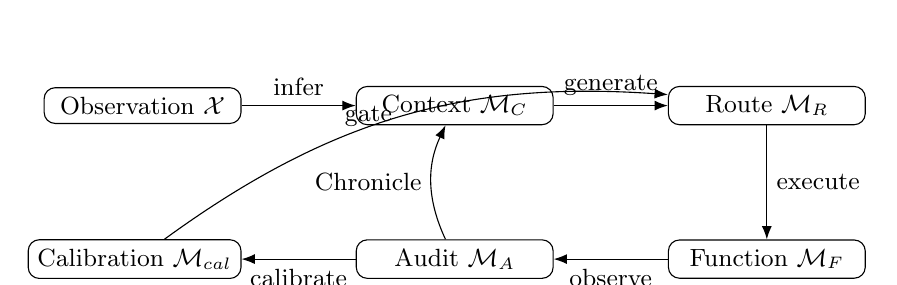
\begin{tikzpicture}[node distance=1.45cm,>=Latex,every node/.style={font=\small}]
\node[draw,rounded corners,minimum width=2.5cm] (x) {Observation $\mathcal{X}$};
\node[draw,rounded corners,right=of x,minimum width=2.5cm] (c) {Context $\M_C$};
\node[draw,rounded corners,right=of c,minimum width=2.5cm] (r) {Route $\M_R$};
\node[draw,rounded corners,below=of r,minimum width=2.5cm] (f) {Function $\M_F$};
\node[draw,rounded corners,left=of f,minimum width=2.5cm] (a) {Audit $\M_A$};
\node[draw,rounded corners,left=of a,minimum width=2.5cm] (cal) {Calibration $\M_{cal}$};
\draw[->] (x)--node[above]{infer} (c);\draw[->] (c)--node[above]{generate} (r);
\draw[->] (r)--node[right]{execute} (f);\draw[->] (f)--node[below]{observe} (a);
\draw[->] (a)--node[below]{calibrate} (cal);\draw[->,bend left=20] (cal) to node[left]{gate} (r);
\draw[->,bend left=25] (a) to node[left]{Chronicle} (c);
\end{tikzpicture}
\caption{G2 couples multiple spaces with distinct semantics and evidence.}
\end{figure}

Each space may carry its own metric. Cross-space maps induce pullbacks. For example, $\Phi:\M_F\to\M_A$ induces $g_F^{audit}=\Phi^*g_A$, measuring only functional variation visible through the audit schema. A router map into the probability simplex can use a stable Hellinger baseline
\begin{equation}
d_H(p,q)=\frac{1}{\sqrt{2}}\lVert\sqrt{p}-\sqrt{q}\rVert_2.
\end{equation}
Fisher--Rao should remain an evaluation metric until gradient stability is demonstrated.

\section{Stable Flow Matching Dynamical Systems as a design pattern}
Perez-Dattari et al. introduce Stable Flow Matching Dynamical Systems, combining expressive multimodal flow matching with positive invariance and Lyapunov stability constraints \cite{perezdattari2026sfmds,lipman2023flow}. The key design is to learn a stochastic vector field while constraining generated velocities to an admissible set. The paper offers soft penalty-based and hard structurally projected variants and extends the construction to Lie groups.

The contribution to MMALS is not the robot application or the flow-matching loss. It is the pattern:
\begin{enumerate}
\item expressive learned dynamics can be restricted to an admissible solution set;
\item safety constraints can be soft or architectural;
\item latent Lyapunov functions may simplify stability conditions;
\item non-Euclidean state spaces should be respected where physically or functionally justified.
\end{enumerate}

The analogy is
\begin{equation}
\dot{x}\in\dot{\mathcal{X}}_A
\quad\Longleftrightarrow\quad
\delta s\in T_s\M^{adm},
\end{equation}
where $s$ is an MMALS state containing route, function, memory, calibration, cost, and audit variables. The admissible tangent cone contains update directions satisfying declared constraints.

The limits matter. SFMDS studies continuous-time trajectories with a defined equilibrium. MMALS studies historical learning systems whose objectives and coordinates can change. G2 must not claim global asymptotic stability unless a meaningful equilibrium or invariant set is defined and the conditions are proved.

A soft constraint adds penalties:
\begin{equation}
L_{G2}=L_{task}+\lambda_RL_{ret}+\lambda_CL_{cost}+\lambda_DL_{drift}+\lambda_AL_{audit}+\lambda_SL_{safe}.
\end{equation}
A hard constraint projects a proposed transition $v$ onto an admissible cone:
\begin{equation}
v^{\Pi}=\Pi_{\mathcal{T}_{adm}(s)}(v).
\end{equation}
Candidate inequalities are
\begin{align}
\Delta\mathrm{Retention}(v)&\ge-\epsilon_R,\\
\Delta\mathrm{Risk}(v)&\le\epsilon_S,\\
\mathrm{Cost}(v)&\le B,\\
\mathrm{AuditVisibility}(v)&\ge\eta_A.
\end{align}
Hard projection is justified only if these quantities can be estimated reliably and projection does not destroy learning.

\section{From route selection to admissible adaptation flow}
The minimal \TPUT state is \cite{mmalstput}
\begin{equation}
s_t=(z_t,\tilde q_t(c),m_t,g_t,D_t,B_t),
\end{equation}
and routes are scored with named components:
\begin{equation}
E(r)=E_{fit}+E_{mem}+E_{ret}+E_{cost}+E_{drift}+E_{spec}+E_{audit}+E_{safe}.
\end{equation}
G2 changes the role of energy. It is not only a ranking score; its local derivatives can define candidate directions while constraints define admissibility.

\subsection{Route--function alignment}
A router may stay smooth while host function drifts. Define
\begin{equation}
A_{r,h}(t)=\mathrm{align}\left(\mathcal{S}_{route,h}(t),\mathcal{S}_{func,h}(t)\right).
\end{equation}
The quantity must be operationally estimated before it can trigger repair. G2-0 compares three estimators.

\paragraph{Intervention estimator.} For perturbations $\delta z_i$, collect functional changes $\delta y_i=f_h(z_i+\delta z_i)-f_h(z_i)$ and estimate a dominant functional subspace by SVD. Estimate the route subspace from local router gradients or route-logit perturbations. Alignment is the mean squared cosine of principal angles:
\begin{equation}
\widehat A^{int}_{r,h}=\frac{1}{k}\sum_{j=1}^{k}\cos^2\theta_j\left(\widehat{\mathcal S}_{route,h},\widehat{\mathcal S}_{func,h}\right).
\end{equation}

\paragraph{Jacobian estimator.} Compare dominant right-singular subspaces of $J_h^q=\partial q_h/\partial z$ and $J_h^f=\partial f_h/\partial z$. This is computationally direct but may be unstable and coordinate-sensitive.

\paragraph{Counterfactual contribution estimator.} Measure host contribution
\begin{equation}
\Delta_h(x)=L(f_{\neg h}(x),y)-L(f(x),y)
\end{equation}
and compare it with route confidence, for example by rank correlation. This is less geometrically pure but more behaviourally grounded.

A repair action requires agreement among behaviour, geometry, and stability diagnostics. Router repair is considered only when oracle-host competence is high, route regret is high, alignment is low, and host function is stable. Host repair is considered when oracle-host competence and functional retention are low while routing remains locally coherent. Otherwise the system abstains from automatic repair and records an indeterminate diagnosis.

\subsection{Counterfactual route regret}
For every admissible route, evaluate frozen execution:
\begin{equation}
R_{route}(x)=L(r_{selected},x)-\min_{r\in\mathcal{R}_{adm}(x)}L(r,x).
\end{equation}
This separates host incapacity from router misallocation. Full counterfactual search is primarily an offline evaluator unless runtime cost is acceptable.

\subsection{Capacity and saturation}
New capacity should be allocated only when evidence separates representational saturation from plasticity saturation. A host creation action is admissible when existing routes have high counterfactual regret, adaptation directions are blocked by justified constraints, and robust calibration rejects current capability. The allocation must be compared with replay, EWC, progressive architectures, and sparse MoE baselines \cite{kirkpatrick2017ewc,shazeer2017moe,fedus2022switch}.

\section{Chronicle as a geometric historical system}
Every reconstructive record should contain
\begin{equation}
A_t=(x_t,z_t,\tilde q_t,R_t,E_t,\pi_t,r_t^*,y_t,g_t,\Gamma_t,\mathrm{cost}_t,\mathrm{version}_t).
\end{equation}
A compiled memory object is a macro-route plus a validity envelope
\begin{equation}
\mu=(r_{macro},\Omega_C,\Omega_F,\Omega_{cal},B_{max},\tau_{expiry},\mathcal{P}).
\end{equation}
The envelope is not merely a ball in latent space. It is the intersection of context, functional, calibration, cost, and provenance conditions.

A transition between capabilities must be evaluated in three relations:
\begin{align}
G_{geom}(i,j)&: \text{representational proximity},\\
G_{func}(i,j)&: \text{functional substitutability or positive transfer},\\
G_{cal}(i,j)&: \text{calibration compatibility}.
\end{align}
A merge is admissible only when the relevant relations support it. Proximity alone is insufficient.

Retirement becomes a value decision:
\begin{equation}
\mathrm{retain}(h)\iff \mathbb{E}[V_{reuse}(h)]>C_{capacity}(h)+C_{interference}(h)+C_{audit}(h).
\end{equation}
The uncertainty of this estimate and any irreversible loss must be recorded.

\section{Safe conformal calibration as a geometric gate}
Conformal prediction supplies finite-sample marginal coverage under stated assumptions \cite{vovk2005algorithmic,angelopoulos2023conformal}. Adaptive conformal inference can respond to shift \cite{gibbs2021adaptive}. Neither is a system safety proof. \CAL is one gate in a layered assurance chain.

For high-confidence context inference,
\begin{equation}
\Gamma_c(x)=\{y:S_c(x,y)\le q_{1-\alpha,c}\}.
\end{equation}
For ambiguous context inference, preserve several plausible contexts and construct a validated robust aggregation
\begin{equation}
\Gamma_{rob}(x)=\mathcal{R}\left(\{\Gamma_c(x):c\in\mathrm{TopK}(q)\}\right).
\end{equation}
This implements non-premature commitment.

CAL should report coverage error, set size, calibration inflation, prediction bias, action and abstention rates, and severity-weighted violations. A calibrator can hide routing failure by widening sets. Chronicle should therefore separate retention failure, inference failure, functional drift, and calibration compensation.

A host may have a calibrated latent acceptance region
\begin{equation}
\mathcal{C}_h=\{z:g_h(z)\le q_{1-\alpha,h}\}.
\end{equation}
An input outside all regions triggers abstention, robust multi-host evaluation, or capacity investigation. Geometric inclusion does not imply functional correctness; host-specific outcomes and interventions remain mandatory.

\subsection{Meta-calibration of the admissibility layer}
The admissibility projector does not observe true retention, risk, cost, or audit visibility. It consumes estimates. Therefore the operational object is not a known safe set $\mathcal A^\star$, but an estimated admissible set $\widehat{\mathcal A}_{1-\alpha}$ whose constituent estimators expose uncertainty and calibration evidence.

For a benefit-like constraint $m(r)\ge m_{min}$, admission uses a conservative lower confidence bound:
\begin{equation}
\mathrm{LCB}_{1-\alpha_m}[m(r)]\ge m_{min}.
\end{equation}
For a harm-like constraint $u(r)\le u_{max}$, admission uses an upper confidence bound:
\begin{equation}
\mathrm{UCB}_{1-\alpha_u}[u(r)]\le u_{max}.
\end{equation}
The gate returns three states: admissible, inadmissible, or indeterminate. Indeterminate means that evidence is insufficient; uncertainty must never be silently converted into permission.

Every gate estimator records its identity, version, training and calibration distributions, empirical coverage, uncertainty width, boundary bias, drift detector, and fallback policy. A nominally hard constraint is demoted to a soft penalty or abstention whenever its estimator cannot maintain the preregistered calibration contract.

Two offline qualification metrics are central. False admissibility measures unsafe optimism:
\begin{equation}
\mathrm{FAR}_{gate}=\Pr\left(r\in\widehat{\mathcal A}_{1-\alpha}\ \wedge\ r\notin\mathcal A^\star\right).
\end{equation}
Gate regret compares the decision induced by the estimated set with an oracle set available only in controlled experiments:
\begin{equation}
\mathrm{GateRegret}=J(r_{\widehat{\mathcal A}})-J(r_{\mathcal A^\star}).
\end{equation}
A calibrated CAL output does not automatically calibrate these upstream estimators. Meta-calibration is an independent assurance layer.

\section{Candidate Lyapunov perspectives}
A Lyapunov-like candidate would measure distance from a desired operational set, not necessarily a point equilibrium:
\begin{equation}
\mathcal{S}_{safe}=\{s:\mathrm{risk}\le\rho,\ \mathrm{retention}\ge R_{min},\ \mathrm{cost}\le B,\ \mathrm{auditability}\ge A_{min}\}.
\end{equation}
A set-stability candidate is $V(s)=d(s,\mathcal{S}_{safe})^2$. An admissible direction may satisfy
\begin{equation}
\nabla V(s)^\top v\le-\kappa V(s)+\xi_t,
\end{equation}
where $\xi_t$ permits controlled adaptation under non-stationarity.

Strict monotonic decrease may be wrong: useful learning can temporarily increase loss, uncertainty, or cost. G2 should examine hard invariance for safety constraints, bounded regret, recovery to acceptable sets, input-to-state stability with drift as disturbance, and multiple Lyapunov functions for different regimes.

The framing is falsified when the candidate does not predict failures, adds no utility, creates severe intransigence, or depends arbitrarily on representation coordinates.

\section{Lie groups, subspaces, Koopman, and mechanics}
SFMDS uses Lie groups because robot orientations genuinely live on $SO(3)$ or $SE(3)$. MMALS should use Lie structure only where a real compositional symmetry exists: invertible route transformations, operator-valued histories, or physical pose applications. A host bank is not automatically a group; closure and inverses may fail.

If context or function is subspace-valued, routing may be studied on a Grassmann manifold. This is admitted only if subspace routing outperforms vector prototypes under equal compute and improves causal intervention specificity.

Koopman methods suggest that nonlinear adaptation trajectories may become simpler in a lifted observable space. Euler--Poincare mechanics suggests constrained evolution under symmetry reduction. Both are mathematical foundations, not implementation mandates. Their value must be measured by prediction, control, or audit of real adaptation trajectories.

\section{Engineering architecture}
A deployable G2 system separates deterministic infrastructure from learned components:
\begin{enumerate}
\item context inference service producing sparse $q(c\mid x,m)$ and uncertainty;
\item route generator enumerating feasible host and memory coalitions;
\item energy evaluator computing named objective and constraint terms;
\item admissibility projector rejecting or projecting unsafe adaptation actions;
\item host executor running selected specialists;
\item CAL service producing sets, diagnostics, and action gates;
\item Chronicle as immutable evidence log and compiled-memory registry;
\item counterfactual auditor for offline route and host interventions;
\item lifecycle manager for create, reuse, merge, repurpose, and retire.
\end{enumerate}

\begin{algorithm}[ht]
\caption{Minimal G2 route and adaptation loop}
\begin{algorithmic}[1]
\Require input $x$, Chronicle $m$, goal $g$, budget $B$
\State $z\gets P_\phi(x)$; $q\gets\mathrm{ContextInferer}(z,m)$
\State $R\gets\mathrm{GenerateRoutes}(\mathrm{TopK}(q),m,g,B)$
\For{$r\in R$}
\State compute energy $E(r)$, constraints $C(r)$, and calibration state $\Gamma(r,x)$
\EndFor
\State $R_{adm}\gets\{r:C(r)\le0\land\Gamma(r,x)\text{ passes}\}$
\State $r^*\gets\mathrm{SimplestAdequateRoute}(R_{adm},E,g,B)$
\State $y\gets\mathrm{Execute}(r^*,x,m)$
\State append complete audit record to $M_R$
\If{compilation gate passes} update $M_S$ with macro-route and validity envelope \EndIf
\State propose lifecycle/update direction $v$ and apply $\Pi_{\mathcal{T}_{adm}}(v)$
\State record rejected and projected actions
\State \Return $y$
\end{algorithmic}
\end{algorithm}

Every output must be reproducible from model version, route candidates, energy decomposition, constraint checks, calibration state, memory reads, and lifecycle writes. An evidence store maps claims to runs, seeds, datasets, and code commits.

\section{Experimental programme and falsification}
\subsection{G2-0: instrumentation before architecture}
Use the current RC2O/MMALS host bank. Add counterfactual route regret, route--function alignment drift, context-specific versus robust CAL, calibration inflation after misrouting, and saturation signals before allocation.

\subsection{G2-1: soft admissibility}
Add penalty-based retention, risk, cost, and audit constraints. Compare against the same architecture without geometry and against validation-selected continual-learning baselines.

\subsection{G2-2: hard projection}
Project route or lifecycle actions into a validated admissible region. Report rejected actions, projection magnitude, accuracy, forgetting, intransigence, latency, and compute.

\subsection{G2-3: geometric transport}
Test learned or analytic transport of capabilities between nearby contexts. Include Euclidean and shuffled-geometry nulls.

\subsection{G2-4: manifold-valued routing}
Only if vector prototypes fail, test subspace or manifold route objects. Require matched-cost gain and cross-seed functional identity.

\begin{longtable}{p{0.25\textwidth}p{0.67\textwidth}}
\toprule Endpoint & Required evidence \\ \midrule
Retention/plasticity & Final average accuracy, forgetting, transfer, intransigence.\\
Context inference & Accuracy where labels exist, route regret, uncertainty, novelty detection.\\
Specialization & Ablation locality, intervention specificity, cross-seed function matching.\\
Geometry & Held-out interpolation, null comparisons, operational gain.\\
CAL safety & Coverage, local undercoverage, set size, inflation, severity-weighted violations.\\
Chronicle utility & Reconstruction fidelity, compilation speedup, envelope failures.\\
Cost & Training and active FLOPs, latency, memory, energy proxy.\\
Auditability & Complete traces, claim manifest, replayability, blind-spot analysis.\\
Meta-calibration & Gate-estimator coverage, false admissibility, gate regret, boundary bias, bootstrap decision instability, and drift response.\\
\bottomrule
\end{longtable}

Core ablations remove route geometry, transport, functional distances, context-conditioned CAL, robust fallback, or audit constraints; freeze router or hosts separately; shuffle context geometry; and compare hard projection with matched-strength soft penalties.

The anti-metaphor safeguards are: no geometry without invariance tests; no stability claim without plasticity; no calibration claim that hides widening; no hidden task label renamed as context; no learned auditor accepted without independent validation; no oracle counterfactual presented as runtime; no Lie or Grassmann machinery without baseline failure; and no irreversible lifecycle action without provenance.

\section{Engineering view}
From an engineering standpoint, G2 is a control and assurance layer around an adaptive system. The primary object is not the manifold; it is the decision contract. Inputs, model state, memory state, objective, and resource budget lead to candidate routes. Deterministic checks and learned estimates classify candidates as admissible or inadmissible. The selected route is executed, calibrated, and audited. Any adaptation is treated as a change request with evidence, impact analysis, and rollback semantics.

The architecture should be modular and nearly decomposable in the sense of Simon \cite{simon1962complexity}. Learned models can propose context, route, and value estimates, but evidence schemas, versioning, hard safety rules, and replay must remain deterministic where possible. Geometry becomes useful when it provides stable interfaces: distances with declared invariances, projections with measurable residuals, and transport maps with validity envelopes.

For deployment, the main engineering artefacts are:
\begin{itemize}
\item a route schema and energy decomposition;
\item a typed Chronicle event model;
\item a constraint and projection API;
\item a calibration evidence contract;
\item an experiment and claim manifest;
\item observability traces connecting specification to evidence;
\item a lifecycle state machine for host and memory objects.
\end{itemize}

\section{A twelve-year-old view}
Imagine a school with several small expert teams. One team understands rotated pictures, another colours, another remembers old rules. A coordinator chooses who should help.

Chronicle is the school's history book. It does not only keep old worksheets. It records which team helped, what was decided, what failed, and which shortcuts are safe to reuse.

Geometry means drawing several maps of the school. One map shows which teams understand similar things. Another shows which teams are safe for a problem. Another shows which shortcuts can be reused. The maps are not always the same.

The SFMDS paper is about a robot that can invent many movements but is not allowed to choose dangerous directions. MMALS G2 borrows the idea: the AI may learn in many ways, but some updates are blocked because they would erase important skills, cost too much, or create an unsafe answer.

A soft rule says, ``That direction is bad; pay a penalty.'' A hard rule says, ``That direction is outside the safe zone; you cannot take it.'' Hard rules are stronger, but they may also stop useful learning, so engineers test both.

Conformal calibration is like the coordinator saying, ``I am not sure enough, so I will give several possible answers or ask for help.'' It is not magic safety. It helps the system know when to slow down, use several teams, or abstain.

The scientific goal is not a beautiful map. The map matters only if the school remembers, learns, saves effort, and avoids bad decisions better than a simpler school.

\section{Reference articles explained through both views}
\subsection{Stable Flow Matching Dynamical Systems}
\textbf{Engineering view.} Learn an expressive vector field, derive admissible velocity sets from invariance or Lyapunov conditions, and enforce them by penalty or structural projection. For MMALS, this is a design pattern for an admissibility layer around routes and lifecycle actions.

\textbf{Twelve-year-old view.} The robot can invent many paths, but a safety fence removes paths that could make it crash. MMALS can put a similar fence around learning steps that would erase useful knowledge.

\subsection{Geometry-MMALS G1}
\textbf{Engineering view.} G1 is the qualification programme: descriptive, predictive, causal, and operational evidence. Route smoothness without function is rejected.

\textbf{Twelve-year-old view.} A colourful map does not prove the teams are different. We switch teams off and swap them to test whether each one really has a special job.

\subsection{MMALS-TPUT and RC2O}
\textbf{Engineering view.} TPUT makes the route a first-class object conditioned on context, memory, goals, and budget. Named energy terms and traces provide transparent control before reinforcement learning.

\textbf{Twelve-year-old view.} The coordinator does not always choose the fastest team. It also thinks about memory, cost, safety, and what will be useful tomorrow.

\subsection{The structural prototype}
\textbf{Engineering view.} Frozen paths provide a structural no-forgetting mechanism under strong assumptions. This proves one memory mechanism, not the complete MMALS ecosystem \cite{mmalsprototype}.


\subsection{Information geometry}
\textbf{Engineering view.} Probability distributions form a manifold. MMALS initially uses this to measure route and audit-distribution change, with stable computational baselines before advanced metrics.


\subsection{Conformal prediction}
\textbf{Engineering view.} Conformal methods turn scores into prediction sets with calibrated marginal error under explicit assumptions. Under drift, thresholds and local diagnostics must adapt.


\subsection{Mixture of experts and continual learning}
\textbf{Engineering view.} MoE supplies sparse capacity and routing; continual learning supplies stability--plasticity benchmarks. MMALS's possible originality is functional memory, route history, ecological contribution, cost, and evidence semantics.


\section{PhD contribution and roadmap}
The doctoral contribution is a theory--engineering programme with four linked outputs:
\begin{enumerate}
\item a multi-space geometric formalization of inferred-context continual functional memory;
\item an admissible-adaptation framework connecting route energy, Chronicle lifecycle, and calibrated action gates;
\item a falsifiable protocol separating retention, inference, allocation, functional drift, and calibration compensation;
\item an auditable implementation with claim-to-artifact traceability.
\end{enumerate}

A successful thesis shows that at least one geometric object or constraint predicts and improves continual-system behaviour beyond strong non-geometric baselines under matched compute. A valuable negative result identifies where geometry fails and establishes simpler engineering rules.

The immediate next experiment is deliberately modest: instrument the current system for route regret, route--function alignment, calibration inflation, and saturation. Only when these diagnostics expose a real geometric control problem should G2 introduce projection, transport, Lie structure, or manifold-valued routing.

\section{Private archive chapter: publication recommendation and release-gate plan}
\status{Guillaume-only working chapter. Retain in the private archive; exclude from any external manuscript unless deliberately rewritten.}

\subsection{Why this snapshot should remain internal}
This package is valuable now as a context-recovery instrument across Guillaume's parallel research, engineering, quantum, identity, and education streams. It freezes vocabulary, hypotheses, boundaries, and the current evidence hierarchy. It should not yet be presented as the canonical G2 specification because the key operational estimators, meta-calibration layer, and G2-0 evidence do not exist at publication quality.

The recommended external publication is not a larger speculative geometry paper. It is a narrower, evidence-backed specification whose central result is the separation of five failure modes: retention failure, context-inference failure, route misallocation, host-functional drift, and calibration compensation. Geometry should enter only where it improves diagnosis or control beyond simpler baselines.

\subsection{Recommended publication sequence}
\begin{enumerate}
\item \textbf{Internal snapshot release.} Archive this v0.2-internal package with commit hash, provenance, reviewer note, and no external claims.
\item \textbf{G2-0 methods note.} Publish only instrumentation definitions: counterfactual route audit, route--function estimators, gate-estimator calibration, and claim schema.
\item \textbf{CAL-compatible hypothesis-verification paper.} Demonstrate the failure decomposition and robust gating on controlled streams before proposing hard geometric projection.
\item \textbf{G2 specification release candidate.} Consolidate only mechanisms that passed preregistered gates, with all deferred geometry moved to a research appendix.
\item \textbf{External paper.} Target a continual-learning, trustworthy-ML, or systems venue with one clear contribution and released artifacts.
\end{enumerate}

\subsection{Detailed action plan before a real specification publication}
\paragraph{Phase P0: repository and provenance freeze.}
Tag the current branch, generate checksums, preserve source PDFs and reviewed digestions, record environment versions, and create a claim manifest mapping each sentence class to evidence status: established, G1-qualified, G2 candidate, or deferred.

\paragraph{Phase P1: G2-0 instrumentation.}
Implement an exhaustive offline host evaluator for each sample. Log selected-host loss, oracle-host loss, route regret, context confidence, host ablation contribution, functional-retention probes, route and function subspaces, CAL set size, coverage, inflation, cost, and audit completeness. No architecture change is allowed in this phase.

\paragraph{Phase P2: estimator qualification.}
For every input to admissibility, specify target quantity, estimator, reference oracle in controlled data, calibration method, confidence or conformal interval, bias near thresholds, sample complexity, and drift behaviour. Use nested splits so the gate is never calibrated and evaluated on the same evidence. Reject estimators that cannot support stable decisions near boundaries.

\paragraph{Phase P3: route--function estimator study.}
Compare intervention, Jacobian, and counterfactual-contribution estimators. Required tests include cross-seed stability, reparameterization sensitivity, bootstrap intervals, intervention specificity, relation to future route regret, and incremental compute. Select no estimator solely for elegance.

\paragraph{Phase P4: CAL-compatible robust hypothesis verification.}
Use controlled context transitions with known ground truth, then hidden-context variants. Compare global CAL, oracle-context CAL, inferred-context CAL, and robust multi-context CAL. Inject router errors and host drift separately. Measure whether CAL correctly exposes failure or hides it through inflation. Add severity-weighted action loss and abstention utility.

\paragraph{Phase P5: meta-calibration gates.}
For each gate estimator, preregister nominal coverage and maximum false-admissibility rate. Test in-distribution, gradual drift, abrupt shift, recurring regimes, novel contexts, and adversarial boundary cases. Estimate GateRegret against the controlled oracle and bootstrap route-decision instability. A hard gate is forbidden until these gates pass on a qualification set untouched by model selection.

\paragraph{Phase P6: soft-admissibility experiment.}
Introduce named penalties only after P1--P5. Compare with unconstrained routing, scalar thresholding, uncertainty-only abstention, replay, EWC, PNN, sparse MoE, and matched-capacity controls. Report accuracy, forgetting, intransigence, route regret, false admissibility, cost, and calibration inflation.

\paragraph{Phase P7: hard projection qualification.}
Test a hard projector only when the soft mechanism shows a stable benefit and the constraint estimators are calibrated. Record projection residual, rejected-action rate, useful-action rejection, unsafe-action acceptance, rollback success, latency, and out-of-distribution behaviour. Hard projection must fail closed or become indeterminate when evidence is missing.

\paragraph{Phase P8: cross-benchmark replication.}
Move from Rotated/Permuted MNIST to SplitCIFAR, CORe50, and at least one engineering stream. Freeze thresholds before qualification. Repeat with multiple seeds, compute-matched baselines, and independent reruns. Functional host identities must be matched across seeds by behaviour rather than raw index.

\paragraph{Phase P9: specification editorialization.}
Rewrite the external specification from the evidence upward. Put validated core first, candidate mechanisms second, and deferred mathematics in an appendix. Remove repeated child-level explanations, retain only Chronicle, admissible adaptation, and estimator uncertainty. Publish a reviewer-response matrix and a machine-readable evidence manifest.

\subsection{CAL-compatible robust process and release gates}
The minimum process is a nested, versioned sequence:
\begin{enumerate}
\item development split for models and diagnostic design;
\item calibration split for CAL and gate-estimator intervals;
\item pilot split for preregistering thresholds and budgets;
\item untouched qualification split for claims;
\item temporal or domain-shift holdout for robustness;
\item independent reproduction from a clean checkout.
\end{enumerate}

The external G2 specification is released only when all mandatory gates pass:
\begin{longtable}{p{0.24\textwidth}p{0.56\textwidth}p{0.12\textwidth}}
\toprule Gate & Criterion & Status now \\ \midrule
R0 Reproducibility & Clean build, seeded runs, immutable configs, artifact hashes. & Partial \\
R1 Diagnostic validity & Route regret and functional probes recover injected failures. & Pending \\
R2 Estimator calibration & Declared interval coverage and acceptable boundary bias. & Pending \\
R3 Meta-calibration & False admissibility and GateRegret below frozen thresholds. & Pending \\
R4 Failure separation & Retention, routing, host drift, and CAL compensation are distinguishable. & Pending \\
R5 Operational gain & Better utility under matched accuracy, cost, memory, and latency budgets. & Pending \\
R6 Safety humility & Hard claims restricted to validated scope; indeterminate and fallback paths tested. & Pending \\
R7 Cross-stream robustness & Repeated on natural and engineering streams across seeds. & Pending \\
R8 Audit completeness & Every decision and claim reconstructable from Chronicle and evidence manifests. & Partial \\
R9 External review readiness & Geometry reviewer, CL reviewer, calibration reviewer, and systems reviewer issues closed. & Pending \\
\bottomrule
\end{longtable}

A failed gate does not force abandonment of MMALS. It determines the correct claim level. For example, failure of R3 permits a soft advisory gate but forbids a hard-admissibility claim. Failure of R5 permits publication as a diagnostic study but not as an operational-control specification.


\subsection{Machine-readable claim governance and contamination controls}
The internal archive now accompanies the prose claim ladder with a machine-readable registry. The registry separates estimators, release gates, execution phases, and claims. A JSON Schema requires every G2-candidate claim to state a falsification test and prevents candidate or deferred claims from being marked externally publication-eligible. A CI validator adds cross-registry controls that are difficult to express in schema alone: gate thresholds must be frozen before a phase uses them; phase dependencies must be complete; consumed data splits must have a completed provenance; estimators may not be selected solely for elegance; and an established or G1-qualified claim may not depend on a gate that has not passed.

Two ordering rules answer the latest internal review. First, route--function estimator selection in P3 is restricted to the development split and must not inspect either the calibration split or the later qualification split. Second, the numeric FAR$_{\mathrm{gate}}$ ceiling and GateRegret bound for R3 must be preregistered and committed before P5 consumes qualification evidence. Checklist gates such as clean-build reproducibility and audit reconstruction may freeze their written criterion at archive time; genuinely quantitative gates remain explicitly unfrozen until a number is justified independently of qualification outcomes.

A passing manifest CI result certifies consistency of the research record, not truth of a scientific claim. Pending gates remain pending. This distinction is essential: the governance mechanism prevents accidental promotion of hypotheses while Guillaume changes context across multiple research programmes, but it cannot substitute for G2-0 experiments or CAL-compatible qualification.

\subsection{Personal publication recommendation}
The strongest eventual publication is likely a two-part contribution. Part one is an empirical methods paper showing that autonomous continual systems require separate measurement of retained competence, context inference, route allocation, functional drift, and calibration compensation. Part two, only if supported, is an admissible-adaptation specification using meta-calibrated gates and Chronicle evidence.

The elegant geometric extensions should remain a programme of hypotheses. They become central only when one of them supplies a measurable advantage: better prediction of interference, more specific repair, lower route regret, safer action selection, or stronger auditability at matched cost. Until then, the Barbaresco principle applies: preserve the structure, remove the ornament, and let evidence decide what deserves to mature.

\section{Conclusion}
MMALS G2 reframes continual learning as the controlled historical evolution of routable functions. Chronicle supplies memory and provenance; inferred-context routing supplies conditional action; TPUT supplies utility and cost; CAL supplies calibrated uncertainty gates; geometry supplies neighbourhoods, directions, transport, and boundaries. The selected SFMDS paper contributes the strongest engineering pattern: expressive learning should occur inside an admissible solution space, with a clear distinction between soft encouragement and hard structural guarantees.

The research discipline remains conservative. No new mathematical layer enters the architecture until simpler diagnostics and controls fail. This keeps G2 a falsifiable engineering programme rather than a geometric metaphor.

\begin{thebibliography}{99}
\bibitem{perezdattari2026sfmds} R. Perez-Dattari, F. Leiva, A. Testa, L. Rozo, J. Ruiz-del-Solar, and N. Jaquier. \emph{Let the Dynamics Flow: Stable Flow Matching Dynamical Systems}. arXiv:2606.03834v2, 2026.
\bibitem{geometrymmalsg1} G. Harbonnier et al. \emph{Geometry-MMALS G1: Research Specification}. MMALS Research Programme technical report and GitHub artifact, 2026.
\bibitem{mmalstput} G. Harbonnier et al. \emph{MMALS-TPUT Specification: Target-conditioned Policy--Utility Transport}. MMALS Research Programme technical specification and GitHub artifact, 2026.
\bibitem{mmalsprototype} G. Harbonnier et al. \emph{MMALS Prototype 0.1: Structural Continual Learning with Functional Routing}. Prototype report and notebook, 2026.
\bibitem{kirkpatrick2017ewc} J. Kirkpatrick et al. Overcoming catastrophic forgetting in neural networks. \emph{PNAS}, 114(13):3521--3526, 2017.
\bibitem{parisi2019cl} G. I. Parisi et al. Continual lifelong learning with neural networks: A review. \emph{Neural Networks}, 113:54--71, 2019.
\bibitem{shazeer2017moe} N. Shazeer et al. Outrageously Large Neural Networks: The Sparsely-Gated Mixture-of-Experts Layer. \emph{ICLR}, 2017.
\bibitem{fedus2022switch} W. Fedus, B. Zoph, and N. Shazeer. Switch Transformers. \emph{JMLR}, 23(120):1--39, 2022.
\bibitem{amari2016information} S.-I. Amari. \emph{Information Geometry and Its Applications}. Springer, 2016.
\bibitem{fisher1925theory} R. A. Fisher. Theory of statistical estimation. \emph{Proceedings of the Cambridge Philosophical Society}, 22:700--725, 1925.
\bibitem{lipman2023flow} Y. Lipman et al. Flow Matching for Generative Modeling. \emph{ICLR}, 2023.
\bibitem{vovk2005algorithmic} V. Vovk, A. Gammerman, and G. Shafer. \emph{Algorithmic Learning in a Random World}. Springer, 2005.
\bibitem{angelopoulos2023conformal} A. N. Angelopoulos and S. Bates. Conformal Prediction: A Gentle Introduction. \emph{Foundations and Trends in Machine Learning}, 16(4):494--591, 2023.
\bibitem{gibbs2021adaptive} I. Gibbs and E. Candes. Adaptive Conformal Inference Under Distribution Shift. \emph{NeurIPS}, 2021.
\bibitem{simon1962complexity} H. A. Simon. The Architecture of Complexity. \emph{Proceedings of the American Philosophical Society}, 106(6):467--482, 1962.
\end{thebibliography}
\end{document}
